\documentclass[1p]{elsarticle_modified}
%\bibliographystyle{elsarticle-num}

%\usepackage[colorlinks]{hyperref}
%\usepackage{abbrmath_seonhwa} %\Abb, \Ascr, \Acal ,\Abf, \Afrak
\usepackage{amsfonts}
\usepackage{amssymb}
\usepackage{amsmath}
\usepackage{amsthm}
\usepackage{scalefnt}
\usepackage{amsbsy}
\usepackage{kotex}
\usepackage{caption}
\usepackage{subfig}
\usepackage{color}
\usepackage{graphicx}
\usepackage{xcolor} %% white, black, red, green, blue, cyan, magenta, yellow
\usepackage{float}
\usepackage{setspace}
\usepackage{hyperref}

\usepackage{tikz}
\usetikzlibrary{arrows}

\usepackage{multirow}
\usepackage{array} % fixed length table
\usepackage{hhline}

%%%%%%%%%%%%%%%%%%%%%
\makeatletter
\renewcommand*\env@matrix[1][\arraystretch]{%
	\edef\arraystretch{#1}%
	\hskip -\arraycolsep
	\let\@ifnextchar\new@ifnextchar
	\array{*\c@MaxMatrixCols c}}
\makeatother %https://tex.stackexchange.com/questions/14071/how-can-i-increase-the-line-spacing-in-a-matrix
%%%%%%%%%%%%%%%

\usepackage[normalem]{ulem}

\newcommand{\msout}[1]{\ifmmode\text{\sout{\ensuremath{#1}}}\else\sout{#1}\fi}
%SOURCE: \msout is \stkout macro in https://tex.stackexchange.com/questions/20609/strikeout-in-math-mode

\newcommand{\cancel}[1]{
	\ifmmode
	{\color{red}\msout{#1}}
	\else
	{\color{red}\sout{#1}}
	\fi
}

\newcommand{\add}[1]{
	{\color{blue}\uwave{#1}}
}

\newcommand{\replace}[2]{
	\ifmmode
	{\color{red}\msout{#1}}{\color{blue}\uwave{#2}}
	\else
	{\color{red}\sout{#1}}{\color{blue}\uwave{#2}}
	\fi
}

\newcommand{\Sol}{\mathcal{S}} %segment
\newcommand{\D}{D} %diagram
\newcommand{\A}{\mathcal{A}} %arc


%%%%%%%%%%%%%%%%%%%%%%%%%%%%%5 test

\def\sl{\operatorname{\textup{SL}}(2,\Cbb)}
\def\psl{\operatorname{\textup{PSL}}(2,\Cbb)}
\def\quan{\mkern 1mu \triangleright \mkern 1mu}

\theoremstyle{definition}
\newtheorem{thm}{Theorem}[section]
\newtheorem{prop}[thm]{Proposition}
\newtheorem{lem}[thm]{Lemma}
\newtheorem{ques}[thm]{Question}
\newtheorem{cor}[thm]{Corollary}
\newtheorem{defn}[thm]{Definition}
\newtheorem{exam}[thm]{Example}
\newtheorem{rmk}[thm]{Remark}
\newtheorem{alg}[thm]{Algorithm}

\newcommand{\I}{\sqrt{-1}}
\begin{document}

%\begin{frontmatter}
%
%\title{Boundary parabolic representations of knots up to 8 crossings}
%
%%% Group authors per affiliation:
%\author{Yunhi Cho} 
%\address{Department of Mathematics, University of Seoul, Seoul, Korea}
%\ead{yhcho@uos.ac.kr}
%
%
%\author{Seonhwa Kim} %\fnref{s_kim}}
%\address{Center for Geometry and Physics, Institute for Basic Science, Pohang, 37673, Korea}
%\ead{ryeona17@ibs.re.kr}
%
%\author{Hyuk Kim}
%\address{Department of Mathematical Sciences, Seoul National University, Seoul 08826, Korea}
%\ead{hyukkim@snu.ac.kr}
%
%\author{Seokbeom Yoon}
%\address{Department of Mathematical Sciences, Seoul National University, Seoul, 08826,  Korea}
%\ead{sbyoon15@snu.ac.kr}
%
%\begin{abstract}
%We find all boundary parabolic representation of knots up to 8 crossings.
%
%\end{abstract}
%\begin{keyword}
%    \MSC[2010] 57M25 
%\end{keyword}
%
%\end{frontmatter}

%\linenumbers
%\tableofcontents
%
\newcommand\colored[1]{\textcolor{white}{\rule[-0.35ex]{0.8em}{1.4ex}}\kern-0.8em\color{red} #1}%
%\newcommand\colored[1]{\textcolor{white}{ #1}\kern-2.17ex	\textcolor{white}{ #1}\kern-1.81ex	\textcolor{white}{ #1}\kern-2.15ex\color{red}#1	}

{\Large $\underline{12a_{0453}~(K12a_{0453})}$}

\setlength{\tabcolsep}{10pt}
\renewcommand{\arraystretch}{1.6}
\vspace{1cm}\begin{tabular}{m{100pt}>{\centering\arraybackslash}m{274pt}}
\multirow{5}{120pt}{
	\centering
	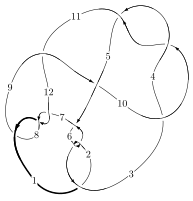
\includegraphics[width=112pt]{../../../GIT/diagram.site/Diagrams/png/1254_12a_0453.png}\\
\ \ \ A knot diagram\footnotemark}&
\allowdisplaybreaks
\textbf{Linearized knot diagam} \\
\cline{2-2}
 &
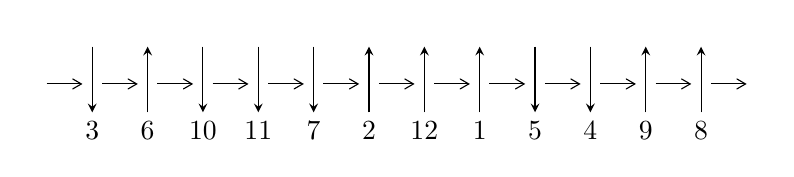
\begin{tikzpicture}[x=20pt, y=17pt]
	% nodes
	\node (C0) at (0, 0) {};
	\node (C1) at (1, 0) {};
	\node (C1U) at (1, +1) {};
	\node (C1D) at (1, -1) {3};

	\node (C2) at (2, 0) {};
	\node (C2U) at (2, +1) {};
	\node (C2D) at (2, -1) {6};

	\node (C3) at (3, 0) {};
	\node (C3U) at (3, +1) {};
	\node (C3D) at (3, -1) {10};

	\node (C4) at (4, 0) {};
	\node (C4U) at (4, +1) {};
	\node (C4D) at (4, -1) {11};

	\node (C5) at (5, 0) {};
	\node (C5U) at (5, +1) {};
	\node (C5D) at (5, -1) {7};

	\node (C6) at (6, 0) {};
	\node (C6U) at (6, +1) {};
	\node (C6D) at (6, -1) {2};

	\node (C7) at (7, 0) {};
	\node (C7U) at (7, +1) {};
	\node (C7D) at (7, -1) {12};

	\node (C8) at (8, 0) {};
	\node (C8U) at (8, +1) {};
	\node (C8D) at (8, -1) {1};

	\node (C9) at (9, 0) {};
	\node (C9U) at (9, +1) {};
	\node (C9D) at (9, -1) {5};

	\node (C10) at (10, 0) {};
	\node (C10U) at (10, +1) {};
	\node (C10D) at (10, -1) {4};

	\node (C11) at (11, 0) {};
	\node (C11U) at (11, +1) {};
	\node (C11D) at (11, -1) {9};

	\node (C12) at (12, 0) {};
	\node (C12U) at (12, +1) {};
	\node (C12D) at (12, -1) {8};
	\node (C13) at (13, 0) {};

	% arrows
	\draw[->,>={angle 60}]
	(C0) edge (C1) (C1) edge (C2) (C2) edge (C3) (C3) edge (C4) (C4) edge (C5) (C5) edge (C6) (C6) edge (C7) (C7) edge (C8) (C8) edge (C9) (C9) edge (C10) (C10) edge (C11) (C11) edge (C12) (C12) edge (C13) ;	\draw[->,>=stealth]
	(C1U) edge (C1D) (C2D) edge (C2U) (C3U) edge (C3D) (C4U) edge (C4D) (C5U) edge (C5D) (C6D) edge (C6U) (C7D) edge (C7U) (C8D) edge (C8U) (C9U) edge (C9D) (C10U) edge (C10D) (C11D) edge (C11U) (C12D) edge (C12U) ;
	\end{tikzpicture} \\
\hhline{~~} \\& 
\textbf{Solving Sequence} \\ \cline{2-2} 
 &
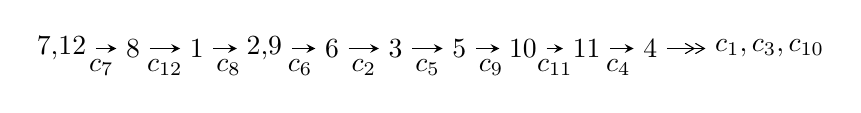
\begin{tikzpicture}[x=23pt, y=7pt]
	% node
	\node (A0) at (-1/8, 0) {7,12};
	\node (A1) at (1, 0) {8};
	\node (A2) at (2, 0) {1};
	\node (A3) at (49/16, 0) {2,9};
	\node (A4) at (33/8, 0) {6};
	\node (A5) at (41/8, 0) {3};
	\node (A6) at (49/8, 0) {5};
	\node (A7) at (57/8, 0) {10};
	\node (A8) at (65/8, 0) {11};
	\node (A9) at (73/8, 0) {4};
	\node (C1) at (1/2, -1) {$c_{7}$};
	\node (C2) at (3/2, -1) {$c_{12}$};
	\node (C3) at (5/2, -1) {$c_{8}$};
	\node (C4) at (29/8, -1) {$c_{6}$};
	\node (C5) at (37/8, -1) {$c_{2}$};
	\node (C6) at (45/8, -1) {$c_{5}$};
	\node (C7) at (53/8, -1) {$c_{9}$};
	\node (C8) at (61/8, -1) {$c_{11}$};
	\node (C9) at (69/8, -1) {$c_{4}$};
	\node (A10) at (11, 0) {$c_{1},c_{3},c_{10}$};

	% edge
	\draw[->,>=stealth]	
	(A0) edge (A1) (A1) edge (A2) (A2) edge (A3) (A3) edge (A4) (A4) edge (A5) (A5) edge (A6) (A6) edge (A7) (A7) edge (A8) (A8) edge (A9) ;
	\draw[->>,>={angle 60}]	
	(A9) edge (A10);
\end{tikzpicture} \\ 

\end{tabular} \\

\footnotetext{
The image of knot diagram is generated by the software ``\textbf{Draw programme}" developed by Andrew Bartholomew(\url{http://www.layer8.co.uk/maths/draw/index.htm\#Running-draw}), where we modified some parts for our purpose(\url{https://github.com/CATsTAILs/LinksPainter}).
}\phantom \\ \newline 
\centering \textbf{Ideals for irreducible components\footnotemark of $X_{\text{par}}$} 
 
\begin{align*}
I^u_{1}&=\langle 
-5.18498\times10^{53} u^{79}+9.21176\times10^{53} u^{78}+\cdots+1.01955\times10^{53} b+2.95698\times10^{54},\\
\phantom{I^u_{1}}&\phantom{= \langle  }-5.89948\times10^{53} u^{79}+1.14051\times10^{54} u^{78}+\cdots+3.56844\times10^{53} a+2.68572\times10^{54},\\
\phantom{I^u_{1}}&\phantom{= \langle  }u^{80}-3 u^{79}+\cdots+39 u+7\rangle \\
I^u_{2}&=\langle 
- a^2+2 b+2 a-1,\;a^4-4 a^3+8 a^2-8 a+7,\;u-1\rangle \\
I^u_{3}&=\langle 
b^2- b+1,\;a+1,\;u+1\rangle \\
\\
\end{align*}
\raggedright * 3 irreducible components of $\dim_{\mathbb{C}}=0$, with total 86 representations.\\
\footnotetext{All coefficients of polynomials are rational numbers. But the coefficients are sometimes approximated in decimal forms when there is not enough margin.}
\newpage
\renewcommand{\arraystretch}{1}
\centering \section*{I. $I^u_{1}= \langle -5.18\times10^{53} u^{79}+9.21\times10^{53} u^{78}+\cdots+1.02\times10^{53} b+2.96\times10^{54},\;-5.90\times10^{53} u^{79}+1.14\times10^{54} u^{78}+\cdots+3.57\times10^{53} a+2.69\times10^{54},\;u^{80}-3 u^{79}+\cdots+39 u+7 \rangle$}
\flushleft \textbf{(i) Arc colorings}\\
\begin{tabular}{m{7pt} m{180pt} m{7pt} m{180pt} }
\flushright $a_{7}=$&$\begin{pmatrix}1\\0\end{pmatrix}$ \\
\flushright $a_{12}=$&$\begin{pmatrix}0\\u\end{pmatrix}$ \\
\flushright $a_{8}=$&$\begin{pmatrix}1\\- u^2\end{pmatrix}$ \\
\flushright $a_{1}=$&$\begin{pmatrix}u\\- u^3+u\end{pmatrix}$ \\
\flushright $a_{2}=$&$\begin{pmatrix}1.65324 u^{79}-3.19611 u^{78}+\cdots-25.8162 u-7.52631\\5.08555 u^{79}-9.03510 u^{78}+\cdots-179.732 u-29.0027\end{pmatrix}$ \\
\flushright $a_{9}=$&$\begin{pmatrix}- u^2+1\\u^4-2 u^2\end{pmatrix}$ \\
\flushright $a_{6}=$&$\begin{pmatrix}3.74801 u^{79}-5.88500 u^{78}+\cdots-176.187 u-27.7131\\-2.52283 u^{79}+4.91016 u^{78}+\cdots+84.4363 u+12.8759\end{pmatrix}$ \\
\flushright $a_{3}=$&$\begin{pmatrix}3.51962 u^{79}-6.36792 u^{78}+\cdots-79.7796 u-13.5372\\-0.545223 u^{79}+0.560292 u^{78}+\cdots+14.1983 u+3.10047\end{pmatrix}$ \\
\flushright $a_{5}=$&$\begin{pmatrix}1.22518 u^{79}-0.974834 u^{78}+\cdots-91.7506 u-14.8372\\-2.52283 u^{79}+4.91016 u^{78}+\cdots+84.4363 u+12.8759\end{pmatrix}$ \\
\flushright $a_{10}=$&$\begin{pmatrix}-1.04068 u^{79}+1.20381 u^{78}+\cdots+93.2953 u+14.9388\\-2.67930 u^{79}+4.50705 u^{78}+\cdots+118.727 u+18.8216\end{pmatrix}$ \\
\flushright $a_{11}=$&$\begin{pmatrix}- u^5+2 u^3- u\\u^7-3 u^5+2 u^3+u\end{pmatrix}$ \\
\flushright $a_{4}=$&$\begin{pmatrix}5.22259 u^{79}-7.87498 u^{78}+\cdots-229.649 u-37.4148\\-5.32240 u^{79}+9.42963 u^{78}+\cdots+159.124 u+25.3193\end{pmatrix}$\\&\end{tabular}
\flushleft \textbf{(ii) Obstruction class $= -1$}\\~\\
\flushleft \textbf{(iii) Cusp Shapes $= 32.2654 u^{79}-56.5988 u^{78}+\cdots-1064.29 u-181.543$}\\~\\
\newpage\renewcommand{\arraystretch}{1}
\flushleft \textbf{(iv) u-Polynomials at the component}\newline \\
\begin{tabular}{m{50pt}|m{274pt}}
Crossings & \hspace{64pt}u-Polynomials at each crossing \\
\hline $$\begin{aligned}c_{1},c_{5}\end{aligned}$$&$\begin{aligned}
&u^{80}+28 u^{79}+\cdots-16 u+1
\end{aligned}$\\
\hline $$\begin{aligned}c_{2},c_{6}\end{aligned}$$&$\begin{aligned}
&u^{80}-2 u^{79}+\cdots+6 u+1
\end{aligned}$\\
\hline $$\begin{aligned}c_{3},c_{4},c_{10}\end{aligned}$$&$\begin{aligned}
&u^{80}- u^{79}+\cdots+12 u+4
\end{aligned}$\\
\hline $$\begin{aligned}c_{7},c_{8},c_{12}\end{aligned}$$&$\begin{aligned}
&u^{80}-3 u^{79}+\cdots+39 u+7
\end{aligned}$\\
\hline $$\begin{aligned}c_{9}\end{aligned}$$&$\begin{aligned}
&u^{80}+3 u^{79}+\cdots-1980 u+44
\end{aligned}$\\
\hline $$\begin{aligned}c_{11}\end{aligned}$$&$\begin{aligned}
&u^{80}+15 u^{79}+\cdots+29696 u+1792
\end{aligned}$\\
\hline
\end{tabular}\\~\\
\newpage\renewcommand{\arraystretch}{1}
\flushleft \textbf{(v) Riley Polynomials at the component}\newline \\
\begin{tabular}{m{50pt}|m{274pt}}
Crossings & \hspace{64pt}Riley Polynomials at each crossing \\
\hline $$\begin{aligned}c_{1},c_{5}\end{aligned}$$&$\begin{aligned}
&y^{80}+52 y^{79}+\cdots-232 y+1
\end{aligned}$\\
\hline $$\begin{aligned}c_{2},c_{6}\end{aligned}$$&$\begin{aligned}
&y^{80}+28 y^{79}+\cdots-16 y+1
\end{aligned}$\\
\hline $$\begin{aligned}c_{3},c_{4},c_{10}\end{aligned}$$&$\begin{aligned}
&y^{80}-75 y^{79}+\cdots+112 y+16
\end{aligned}$\\
\hline $$\begin{aligned}c_{7},c_{8},c_{12}\end{aligned}$$&$\begin{aligned}
&y^{80}-69 y^{79}+\cdots+887 y+49
\end{aligned}$\\
\hline $$\begin{aligned}c_{9}\end{aligned}$$&$\begin{aligned}
&y^{80}-15 y^{79}+\cdots-3730320 y+1936
\end{aligned}$\\
\hline $$\begin{aligned}c_{11}\end{aligned}$$&$\begin{aligned}
&y^{80}+29 y^{79}+\cdots-17334272 y+3211264
\end{aligned}$\\
\hline
\end{tabular}\\~\\
\newpage\flushleft \textbf{(vi) Complex Volumes and Cusp Shapes}
$$\begin{array}{c|c|c}  
\text{Solutions to }I^u_{1}& \I (\text{vol} + \sqrt{-1}CS) & \text{Cusp shape}\\
 \hline 
\begin{aligned}
u &= \phantom{-}0.935308 + 0.435305 I \\
a &= \phantom{-}0.630371 - 0.162057 I \\
b &= -0.660075 + 0.935719 I\end{aligned}
 & \phantom{-}2.61436 - 3.12647 I & \phantom{-0.000000 } 0 \\ \hline\begin{aligned}
u &= \phantom{-}0.935308 - 0.435305 I \\
a &= \phantom{-}0.630371 + 0.162057 I \\
b &= -0.660075 - 0.935719 I\end{aligned}
 & \phantom{-}2.61436 + 3.12647 I & \phantom{-0.000000 } 0 \\ \hline\begin{aligned}
u &= \phantom{-}0.796363 + 0.441945 I \\
a &= \phantom{-}1.309720 - 0.265298 I \\
b &= -0.680200 - 0.780701 I\end{aligned}
 & \phantom{-}3.09872 + 2.06011 I & \phantom{-0.000000 } 0 \\ \hline\begin{aligned}
u &= \phantom{-}0.796363 - 0.441945 I \\
a &= \phantom{-}1.309720 + 0.265298 I \\
b &= -0.680200 + 0.780701 I\end{aligned}
 & \phantom{-}3.09872 - 2.06011 I & \phantom{-0.000000 } 0 \\ \hline\begin{aligned}
u &= -0.189528 + 0.882751 I \\
a &= -1.09473 - 1.20457 I \\
b &= \phantom{-}0.690554 - 1.030640 I\end{aligned}
 & -5.17726 - 11.04350 I & \phantom{-0.000000 } 0 \\ \hline\begin{aligned}
u &= -0.189528 - 0.882751 I \\
a &= -1.09473 + 1.20457 I \\
b &= \phantom{-}0.690554 + 1.030640 I\end{aligned}
 & -5.17726 + 11.04350 I & \phantom{-0.000000 } 0 \\ \hline\begin{aligned}
u &= -1.011710 + 0.480638 I \\
a &= -1.133710 - 0.245043 I \\
b &= \phantom{-}0.725723 - 0.676763 I\end{aligned}
 & -1.53219 + 0.73845 I & \phantom{-0.000000 } 0 \\ \hline\begin{aligned}
u &= -1.011710 - 0.480638 I \\
a &= -1.133710 + 0.245043 I \\
b &= \phantom{-}0.725723 + 0.676763 I\end{aligned}
 & -1.53219 - 0.73845 I & \phantom{-0.000000 } 0 \\ \hline\begin{aligned}
u &= -0.212777 + 0.844785 I \\
a &= -0.020548 - 0.158541 I \\
b &= \phantom{-}0.789018 + 0.625628 I\end{aligned}
 & -3.96644 - 5.45425 I & \phantom{-0.000000 } 0 \\ \hline\begin{aligned}
u &= -0.212777 - 0.844785 I \\
a &= -0.020548 + 0.158541 I \\
b &= \phantom{-}0.789018 - 0.625628 I\end{aligned}
 & -3.96644 + 5.45425 I & \phantom{-0.000000 } 0\\
 \hline 
 \end{array}$$\newpage$$\begin{array}{c|c|c}  
\text{Solutions to }I^u_{1}& \I (\text{vol} + \sqrt{-1}CS) & \text{Cusp shape}\\
 \hline 
\begin{aligned}
u &= \phantom{-}0.230270 + 0.805111 I \\
a &= \phantom{-}1.23350 - 1.18135 I \\
b &= -0.683422 - 1.002370 I\end{aligned}
 & \phantom{-}0.43105 + 7.58116 I & \phantom{-0.000000 } 0. - 8.40866 I \\ \hline\begin{aligned}
u &= \phantom{-}0.230270 - 0.805111 I \\
a &= \phantom{-}1.23350 + 1.18135 I \\
b &= -0.683422 + 1.002370 I\end{aligned}
 & \phantom{-}0.43105 - 7.58116 I & \phantom{-0.000000 -}0. + 8.40866 I \\ \hline\begin{aligned}
u &= -0.618703 + 0.562447 I \\
a &= -0.403548 - 0.367487 I \\
b &= \phantom{-}0.705780 + 0.826705 I\end{aligned}
 & \phantom{-}0.100507 + 0.533058 I & \phantom{-0.000000 } 0 \\ \hline\begin{aligned}
u &= -0.618703 - 0.562447 I \\
a &= -0.403548 + 0.367487 I \\
b &= \phantom{-}0.705780 - 0.826705 I\end{aligned}
 & \phantom{-}0.100507 - 0.533058 I & \phantom{-0.000000 } 0 \\ \hline\begin{aligned}
u &= -0.569488 + 0.611464 I \\
a &= -1.42307 - 0.59607 I \\
b &= \phantom{-}0.707294 - 0.877786 I\end{aligned}
 & -0.04800 - 4.87101 I & \phantom{-0.000000 -}0. + 6.91200 I \\ \hline\begin{aligned}
u &= -0.569488 - 0.611464 I \\
a &= -1.42307 + 0.59607 I \\
b &= \phantom{-}0.707294 + 0.877786 I\end{aligned}
 & -0.04800 + 4.87101 I & \phantom{-0.000000 } 0. - 6.91200 I \\ \hline\begin{aligned}
u &= -1.074410 + 0.502940 I \\
a &= -0.588936 - 0.064477 I \\
b &= \phantom{-}0.678298 + 0.993914 I\end{aligned}
 & -2.48323 + 6.12770 I & \phantom{-0.000000 } 0 \\ \hline\begin{aligned}
u &= -1.074410 - 0.502940 I \\
a &= -0.588936 + 0.064477 I \\
b &= \phantom{-}0.678298 - 0.993914 I\end{aligned}
 & -2.48323 - 6.12770 I & \phantom{-0.000000 } 0 \\ \hline\begin{aligned}
u &= -0.103875 + 0.802998 I \\
a &= \phantom{-}0.00658 + 1.73987 I \\
b &= -0.067956 + 1.091330 I\end{aligned}
 & -10.00530 - 4.77646 I & -9.45758 + 3.89445 I \\ \hline\begin{aligned}
u &= -0.103875 - 0.802998 I \\
a &= \phantom{-}0.00658 - 1.73987 I \\
b &= -0.067956 - 1.091330 I\end{aligned}
 & -10.00530 + 4.77646 I & -9.45758 - 3.89445 I\\
 \hline 
 \end{array}$$\newpage$$\begin{array}{c|c|c}  
\text{Solutions to }I^u_{1}& \I (\text{vol} + \sqrt{-1}CS) & \text{Cusp shape}\\
 \hline 
\begin{aligned}
u &= -0.787931 + 0.048490 I \\
a &= -0.705941 + 0.065873 I \\
b &= -0.281416 - 0.032919 I\end{aligned}
 & -3.20361 + 0.00081 I & -1.068722 + 0.283561 I \\ \hline\begin{aligned}
u &= -0.787931 - 0.048490 I \\
a &= -0.705941 - 0.065873 I \\
b &= -0.281416 + 0.032919 I\end{aligned}
 & -3.20361 - 0.00081 I & -1.068722 - 0.283561 I \\ \hline\begin{aligned}
u &= \phantom{-}0.266680 + 0.740721 I \\
a &= \phantom{-}0.020003 - 0.258774 I \\
b &= -0.741730 + 0.664409 I\end{aligned}
 & \phantom{-}1.44053 + 2.13306 I & \phantom{-}2.30999 - 3.70879 I \\ \hline\begin{aligned}
u &= \phantom{-}0.266680 - 0.740721 I \\
a &= \phantom{-}0.020003 + 0.258774 I \\
b &= -0.741730 - 0.664409 I\end{aligned}
 & \phantom{-}1.44053 - 2.13306 I & \phantom{-}2.30999 + 3.70879 I \\ \hline\begin{aligned}
u &= -1.159110 + 0.364671 I \\
a &= -1.146160 - 0.714549 I \\
b &= -0.019630 - 1.019000 I\end{aligned}
 & -6.79020 + 0.55303 I & \phantom{-0.000000 } 0 \\ \hline\begin{aligned}
u &= -1.159110 - 0.364671 I \\
a &= -1.146160 + 0.714549 I \\
b &= -0.019630 + 1.019000 I\end{aligned}
 & -6.79020 - 0.55303 I & \phantom{-0.000000 } 0 \\ \hline\begin{aligned}
u &= -1.225370 + 0.147900 I \\
a &= -0.780791 + 0.104181 I \\
b &= \phantom{-}0.498165 + 1.025250 I\end{aligned}
 & \phantom{-}2.35150 + 1.12565 I & \phantom{-0.000000 } 0 \\ \hline\begin{aligned}
u &= -1.225370 - 0.147900 I \\
a &= -0.780791 - 0.104181 I \\
b &= \phantom{-}0.498165 - 1.025250 I\end{aligned}
 & \phantom{-}2.35150 - 1.12565 I & \phantom{-0.000000 } 0 \\ \hline\begin{aligned}
u &= \phantom{-}1.204440 + 0.280604 I \\
a &= \phantom{-}1.085160 - 0.510984 I \\
b &= -0.091913 - 0.991633 I\end{aligned}
 & -0.58135 + 1.79490 I & \phantom{-0.000000 } 0 \\ \hline\begin{aligned}
u &= \phantom{-}1.204440 - 0.280604 I \\
a &= \phantom{-}1.085160 + 0.510984 I \\
b &= -0.091913 + 0.991633 I\end{aligned}
 & -0.58135 - 1.79490 I & \phantom{-0.000000 } 0\\
 \hline 
 \end{array}$$\newpage$$\begin{array}{c|c|c}  
\text{Solutions to }I^u_{1}& \I (\text{vol} + \sqrt{-1}CS) & \text{Cusp shape}\\
 \hline 
\begin{aligned}
u &= \phantom{-}1.24271\phantom{ +0.000000I} \\
a &= \phantom{-}1.03607\phantom{ +0.000000I} \\
b &= -0.509667\phantom{ +0.000000I}\end{aligned}
 & \phantom{-}2.60848\phantom{ +0.000000I} & \phantom{-0.000000 } 0 \\ \hline\begin{aligned}
u &= -1.253110 + 0.182081 I \\
a &= \phantom{-}0.73377 + 2.17860 I \\
b &= -0.682535 - 0.698735 I\end{aligned}
 & -2.04164 + 0.28284 I & \phantom{-0.000000 } 0 \\ \hline\begin{aligned}
u &= -1.253110 - 0.182081 I \\
a &= \phantom{-}0.73377 - 2.17860 I \\
b &= -0.682535 + 0.698735 I\end{aligned}
 & -2.04164 - 0.28284 I & \phantom{-0.000000 } 0 \\ \hline\begin{aligned}
u &= \phantom{-}0.057893 + 0.724540 I \\
a &= \phantom{-}0.02131 + 1.71614 I \\
b &= \phantom{-}0.042565 + 1.034450 I\end{aligned}
 & -4.07583 + 1.86281 I & -6.38175 - 4.14946 I \\ \hline\begin{aligned}
u &= \phantom{-}0.057893 - 0.724540 I \\
a &= \phantom{-}0.02131 - 1.71614 I \\
b &= \phantom{-}0.042565 - 1.034450 I\end{aligned}
 & -4.07583 - 1.86281 I & -6.38175 + 4.14946 I \\ \hline\begin{aligned}
u &= \phantom{-}1.301140 + 0.047924 I \\
a &= \phantom{-}0.851162 - 0.262258 I \\
b &= -0.353950 - 1.049460 I\end{aligned}
 & -0.52296 + 3.40294 I & \phantom{-0.000000 } 0 \\ \hline\begin{aligned}
u &= \phantom{-}1.301140 - 0.047924 I \\
a &= \phantom{-}0.851162 + 0.262258 I \\
b &= -0.353950 + 1.049460 I\end{aligned}
 & -0.52296 - 3.40294 I & \phantom{-0.000000 } 0 \\ \hline\begin{aligned}
u &= -1.278660 + 0.248936 I \\
a &= \phantom{-}3.06357 + 0.27921 I \\
b &= -0.663651 + 0.979925 I\end{aligned}
 & -2.89654 - 4.94761 I & \phantom{-0.000000 } 0 \\ \hline\begin{aligned}
u &= -1.278660 - 0.248936 I \\
a &= \phantom{-}3.06357 - 0.27921 I \\
b &= -0.663651 - 0.979925 I\end{aligned}
 & -2.89654 + 4.94761 I & \phantom{-0.000000 } 0 \\ \hline\begin{aligned}
u &= \phantom{-}1.291440 + 0.263515 I \\
a &= \phantom{-}0.690783 + 0.098744 I \\
b &= -0.552614 + 1.074470 I\end{aligned}
 & -2.71721 + 1.66465 I & \phantom{-0.000000 } 0\\
 \hline 
 \end{array}$$\newpage$$\begin{array}{c|c|c}  
\text{Solutions to }I^u_{1}& \I (\text{vol} + \sqrt{-1}CS) & \text{Cusp shape}\\
 \hline 
\begin{aligned}
u &= \phantom{-}1.291440 - 0.263515 I \\
a &= \phantom{-}0.690783 - 0.098744 I \\
b &= -0.552614 - 1.074470 I\end{aligned}
 & -2.71721 - 1.66465 I & \phantom{-0.000000 } 0 \\ \hline\begin{aligned}
u &= -0.150748 + 0.661001 I \\
a &= -0.239366 + 0.050399 I \\
b &= -0.636156 + 0.406125 I\end{aligned}
 & -5.24145 - 3.04676 I & -3.68290 + 3.88325 I \\ \hline\begin{aligned}
u &= -0.150748 - 0.661001 I \\
a &= -0.239366 - 0.050399 I \\
b &= -0.636156 - 0.406125 I\end{aligned}
 & -5.24145 + 3.04676 I & -3.68290 - 3.88325 I \\ \hline\begin{aligned}
u &= \phantom{-}1.32459\phantom{ +0.000000I} \\
a &= \phantom{-}1.00826\phantom{ +0.000000I} \\
b &= -0.636706\phantom{ +0.000000I}\end{aligned}
 & \phantom{-}2.55061\phantom{ +0.000000I} & \phantom{-0.000000 } 0 \\ \hline\begin{aligned}
u &= -0.192008 + 0.640756 I \\
a &= -1.55726 - 1.32579 I \\
b &= \phantom{-}0.639720 - 0.972486 I\end{aligned}
 & -0.54467 - 3.78067 I & -2.80718 + 2.65962 I \\ \hline\begin{aligned}
u &= -0.192008 - 0.640756 I \\
a &= -1.55726 + 1.32579 I \\
b &= \phantom{-}0.639720 + 0.972486 I\end{aligned}
 & -0.54467 + 3.78067 I & -2.80718 - 2.65962 I \\ \hline\begin{aligned}
u &= -1.301240 + 0.293419 I \\
a &= -0.927140 - 0.527970 I \\
b &= \phantom{-}0.131001 - 1.090690 I\end{aligned}
 & \phantom{-}0.16791 - 5.53918 I & \phantom{-0.000000 } 0 \\ \hline\begin{aligned}
u &= -1.301240 - 0.293419 I \\
a &= -0.927140 + 0.527970 I \\
b &= \phantom{-}0.131001 + 1.090690 I\end{aligned}
 & \phantom{-}0.16791 + 5.53918 I & \phantom{-0.000000 } 0 \\ \hline\begin{aligned}
u &= -1.325140 + 0.190326 I \\
a &= -1.008040 - 0.071508 I \\
b &= \phantom{-}0.691635 - 0.250001 I\end{aligned}
 & \phantom{-}4.56651 - 3.15280 I & \phantom{-0.000000 } 0 \\ \hline\begin{aligned}
u &= -1.325140 - 0.190326 I \\
a &= -1.008040 + 0.071508 I \\
b &= \phantom{-}0.691635 + 0.250001 I\end{aligned}
 & \phantom{-}4.56651 + 3.15280 I & \phantom{-0.000000 } 0\\
 \hline 
 \end{array}$$\newpage$$\begin{array}{c|c|c}  
\text{Solutions to }I^u_{1}& \I (\text{vol} + \sqrt{-1}CS) & \text{Cusp shape}\\
 \hline 
\begin{aligned}
u &= -0.018029 + 0.660145 I \\
a &= \phantom{-}1.26111 - 1.82685 I \\
b &= -0.594114 - 1.016650 I\end{aligned}
 & -6.81361 + 1.68208 I & -6.85681 - 2.22241 I \\ \hline\begin{aligned}
u &= -0.018029 - 0.660145 I \\
a &= \phantom{-}1.26111 + 1.82685 I \\
b &= -0.594114 + 1.016650 I\end{aligned}
 & -6.81361 - 1.68208 I & -6.85681 + 2.22241 I \\ \hline\begin{aligned}
u &= \phantom{-}1.345210 + 0.277688 I \\
a &= \phantom{-}0.996087 - 0.105982 I \\
b &= -0.759916 - 0.328235 I\end{aligned}
 & -0.53214 + 6.49202 I & \phantom{-0.000000 } 0 \\ \hline\begin{aligned}
u &= \phantom{-}1.345210 - 0.277688 I \\
a &= \phantom{-}0.996087 + 0.105982 I \\
b &= -0.759916 + 0.328235 I\end{aligned}
 & -0.53214 - 6.49202 I & \phantom{-0.000000 } 0 \\ \hline\begin{aligned}
u &= \phantom{-}1.333900 + 0.342685 I \\
a &= \phantom{-}0.875466 - 0.582857 I \\
b &= -0.106119 - 1.138050 I\end{aligned}
 & -5.48737 + 8.90152 I & \phantom{-0.000000 } 0 \\ \hline\begin{aligned}
u &= \phantom{-}1.333900 - 0.342685 I \\
a &= \phantom{-}0.875466 + 0.582857 I \\
b &= -0.106119 + 1.138050 I\end{aligned}
 & -5.48737 - 8.90152 I & \phantom{-0.000000 } 0 \\ \hline\begin{aligned}
u &= \phantom{-}1.373660 + 0.225693 I \\
a &= -0.91497 + 1.44154 I \\
b &= \phantom{-}0.784938 - 0.698652 I\end{aligned}
 & \phantom{-}5.34197 + 1.50444 I & \phantom{-0.000000 } 0 \\ \hline\begin{aligned}
u &= \phantom{-}1.373660 - 0.225693 I \\
a &= -0.91497 - 1.44154 I \\
b &= \phantom{-}0.784938 + 0.698652 I\end{aligned}
 & \phantom{-}5.34197 - 1.50444 I & \phantom{-0.000000 } 0 \\ \hline\begin{aligned}
u &= \phantom{-}1.373070 + 0.272297 I \\
a &= -2.49390 + 0.15890 I \\
b &= \phantom{-}0.709636 + 0.998983 I\end{aligned}
 & \phantom{-}4.42932 + 7.15478 I & \phantom{-0.000000 } 0 \\ \hline\begin{aligned}
u &= \phantom{-}1.373070 - 0.272297 I \\
a &= -2.49390 - 0.15890 I \\
b &= \phantom{-}0.709636 - 0.998983 I\end{aligned}
 & \phantom{-}4.42932 - 7.15478 I & \phantom{-0.000000 } 0\\
 \hline 
 \end{array}$$\newpage$$\begin{array}{c|c|c}  
\text{Solutions to }I^u_{1}& \I (\text{vol} + \sqrt{-1}CS) & \text{Cusp shape}\\
 \hline 
\begin{aligned}
u &= -1.40021 + 0.29892 I \\
a &= \phantom{-}0.73966 + 1.22831 I \\
b &= -0.826565 - 0.658485 I\end{aligned}
 & \phantom{-}6.72479 - 5.90072 I & \phantom{-0.000000 } 0 \\ \hline\begin{aligned}
u &= -1.40021 - 0.29892 I \\
a &= \phantom{-}0.73966 - 1.22831 I \\
b &= -0.826565 + 0.658485 I\end{aligned}
 & \phantom{-}6.72479 + 5.90072 I & \phantom{-0.000000 } 0 \\ \hline\begin{aligned}
u &= -1.39785 + 0.33105 I \\
a &= \phantom{-}2.28662 + 0.34323 I \\
b &= -0.716310 + 1.030440 I\end{aligned}
 & \phantom{-}5.59576 - 11.68240 I & \phantom{-0.000000 } 0 \\ \hline\begin{aligned}
u &= -1.39785 - 0.33105 I \\
a &= \phantom{-}2.28662 - 0.34323 I \\
b &= -0.716310 - 1.030440 I\end{aligned}
 & \phantom{-}5.59576 + 11.68240 I & \phantom{-0.000000 } 0 \\ \hline\begin{aligned}
u &= \phantom{-}1.39606 + 0.35207 I \\
a &= -0.618370 + 1.142030 I \\
b &= \phantom{-}0.843709 - 0.622934 I\end{aligned}
 & \phantom{-}1.13138 + 9.76187 I & \phantom{-0.000000 } 0 \\ \hline\begin{aligned}
u &= \phantom{-}1.39606 - 0.35207 I \\
a &= -0.618370 - 1.142030 I \\
b &= \phantom{-}0.843709 + 0.622934 I\end{aligned}
 & \phantom{-}1.13138 - 9.76187 I & \phantom{-0.000000 } 0 \\ \hline\begin{aligned}
u &= \phantom{-}1.39337 + 0.37541 I \\
a &= -2.20827 + 0.49155 I \\
b &= \phantom{-}0.709809 + 1.051400 I\end{aligned}
 & -0.1684 + 15.5626 I & \phantom{-0.000000 } 0 \\ \hline\begin{aligned}
u &= \phantom{-}1.39337 - 0.37541 I \\
a &= -2.20827 - 0.49155 I \\
b &= \phantom{-}0.709809 - 1.051400 I\end{aligned}
 & -0.1684 - 15.5626 I & \phantom{-0.000000 } 0 \\ \hline\begin{aligned}
u &= \phantom{-}1.45673 + 0.06706 I \\
a &= -1.57725 + 1.11214 I \\
b &= \phantom{-}0.800472 - 0.820840 I\end{aligned}
 & \phantom{-}6.99812 + 1.19577 I & \phantom{-0.000000 } 0 \\ \hline\begin{aligned}
u &= \phantom{-}1.45673 - 0.06706 I \\
a &= -1.57725 - 1.11214 I \\
b &= \phantom{-}0.800472 + 0.820840 I\end{aligned}
 & \phantom{-}6.99812 - 1.19577 I & \phantom{-0.000000 } 0\\
 \hline 
 \end{array}$$\newpage$$\begin{array}{c|c|c}  
\text{Solutions to }I^u_{1}& \I (\text{vol} + \sqrt{-1}CS) & \text{Cusp shape}\\
 \hline 
\begin{aligned}
u &= \phantom{-}1.46037 + 0.10688 I \\
a &= -2.08437 - 0.58760 I \\
b &= \phantom{-}0.774088 + 0.921625 I\end{aligned}
 & \phantom{-}6.69269 + 7.09251 I & \phantom{-0.000000 } 0 \\ \hline\begin{aligned}
u &= \phantom{-}1.46037 - 0.10688 I \\
a &= -2.08437 + 0.58760 I \\
b &= \phantom{-}0.774088 - 0.921625 I\end{aligned}
 & \phantom{-}6.69269 - 7.09251 I & \phantom{-0.000000 } 0 \\ \hline\begin{aligned}
u &= -1.46462 + 0.02186 I \\
a &= \phantom{-}1.86638 - 0.87686 I \\
b &= -0.789181 + 0.874587 I\end{aligned}
 & \phantom{-}10.49570 - 2.95503 I & \phantom{-0.000000 } 0 \\ \hline\begin{aligned}
u &= -1.46462 - 0.02186 I \\
a &= \phantom{-}1.86638 + 0.87686 I \\
b &= -0.789181 - 0.874587 I\end{aligned}
 & \phantom{-}10.49570 + 2.95503 I & \phantom{-0.000000 } 0 \\ \hline\begin{aligned}
u &= -0.228484 + 0.437922 I \\
a &= \phantom{-}0.219585 - 0.751726 I \\
b &= \phantom{-}0.600073 + 0.715905 I\end{aligned}
 & \phantom{-}0.276256 + 1.175000 I & -2.28134 - 3.06853 I \\ \hline\begin{aligned}
u &= -0.228484 - 0.437922 I \\
a &= \phantom{-}0.219585 + 0.751726 I \\
b &= \phantom{-}0.600073 - 0.715905 I\end{aligned}
 & \phantom{-}0.276256 - 1.175000 I & -2.28134 + 3.06853 I \\ \hline\begin{aligned}
u &= \phantom{-}0.164199 + 0.364320 I \\
a &= \phantom{-}0.313161 + 0.253667 I \\
b &= \phantom{-}0.314435 + 0.339122 I\end{aligned}
 & \phantom{-}0.038038 + 0.896508 I & \phantom{-}0.98315 - 7.41629 I \\ \hline\begin{aligned}
u &= \phantom{-}0.164199 - 0.364320 I \\
a &= \phantom{-}0.313161 - 0.253667 I \\
b &= \phantom{-}0.314435 - 0.339122 I\end{aligned}
 & \phantom{-}0.038038 - 0.896508 I & \phantom{-}0.98315 + 7.41629 I \\ \hline\begin{aligned}
u &= -0.200756 + 0.298050 I \\
a &= -1.72839 + 2.08553 I \\
b &= -0.356274 + 0.854401 I\end{aligned}
 & -5.18017 - 2.38847 I & -8.45347 + 4.78125 I \\ \hline\begin{aligned}
u &= -0.200756 - 0.298050 I \\
a &= -1.72839 - 2.08553 I \\
b &= -0.356274 - 0.854401 I\end{aligned}
 & -5.18017 + 2.38847 I & -8.45347 - 4.78125 I\\
 \hline 
 \end{array}$$\newpage\newpage\renewcommand{\arraystretch}{1}
\centering \section*{II. $I^u_{2}= \langle - a^2+2 b+2 a-1,\;a^4-4 a^3+8 a^2-8 a+7,\;u-1 \rangle$}
\flushleft \textbf{(i) Arc colorings}\\
\begin{tabular}{m{7pt} m{180pt} m{7pt} m{180pt} }
\flushright $a_{7}=$&$\begin{pmatrix}1\\0\end{pmatrix}$ \\
\flushright $a_{12}=$&$\begin{pmatrix}0\\1\end{pmatrix}$ \\
\flushright $a_{8}=$&$\begin{pmatrix}1\\-1\end{pmatrix}$ \\
\flushright $a_{1}=$&$\begin{pmatrix}1\\0\end{pmatrix}$ \\
\flushright $a_{2}=$&$\begin{pmatrix}a\\\frac{1}{2} a^2- a+\frac{1}{2}\end{pmatrix}$ \\
\flushright $a_{9}=$&$\begin{pmatrix}0\\-1\end{pmatrix}$ \\
\flushright $a_{6}=$&$\begin{pmatrix}\frac{1}{2} a^3- a^2+\frac{1}{2} a+1\\-\frac{1}{2} a^2+a-\frac{3}{2}\end{pmatrix}$ \\
\flushright $a_{3}=$&$\begin{pmatrix}-\frac{1}{2} a^3+\frac{3}{2} a^2-\frac{3}{2} a+\frac{1}{2}\\\frac{1}{2} a^2- a+\frac{3}{2}\end{pmatrix}$ \\
\flushright $a_{5}=$&$\begin{pmatrix}\frac{1}{2} a^3-\frac{3}{2} a^2+\frac{3}{2} a-\frac{1}{2}\\-\frac{1}{2} a^2+a-\frac{3}{2}\end{pmatrix}$ \\
\flushright $a_{10}=$&$\begin{pmatrix}2\\a-2\end{pmatrix}$ \\
\flushright $a_{11}=$&$\begin{pmatrix}0\\1\end{pmatrix}$ \\
\flushright $a_{4}=$&$\begin{pmatrix}\frac{1}{2} a^3-\frac{3}{2} a^2+\frac{3}{2} a-\frac{1}{2}\\-\frac{1}{2} a^3+a^2-\frac{1}{2} a-1\end{pmatrix}$\\&\end{tabular}
\flushleft \textbf{(ii) Obstruction class $= 1$}\\~\\
\flushleft \textbf{(iii) Cusp Shapes $= 2 a^2-4 a+2$}\\~\\
\newpage\renewcommand{\arraystretch}{1}
\flushleft \textbf{(iv) u-Polynomials at the component}\newline \\
\begin{tabular}{m{50pt}|m{274pt}}
Crossings & \hspace{64pt}u-Polynomials at each crossing \\
\hline $$\begin{aligned}c_{1},c_{2},c_{5}\end{aligned}$$&$\begin{aligned}
&(u^2- u+1)^2
\end{aligned}$\\
\hline $$\begin{aligned}c_{3},c_{4},c_{9}\\c_{10}\end{aligned}$$&$\begin{aligned}
&(u^2-2)^2
\end{aligned}$\\
\hline $$\begin{aligned}c_{6}\end{aligned}$$&$\begin{aligned}
&(u^2+u+1)^2
\end{aligned}$\\
\hline $$\begin{aligned}c_{7},c_{8}\end{aligned}$$&$\begin{aligned}
&(u-1)^4
\end{aligned}$\\
\hline $$\begin{aligned}c_{11}\end{aligned}$$&$\begin{aligned}
&u^4
\end{aligned}$\\
\hline $$\begin{aligned}c_{12}\end{aligned}$$&$\begin{aligned}
&(u+1)^4
\end{aligned}$\\
\hline
\end{tabular}\\~\\
\newpage\renewcommand{\arraystretch}{1}
\flushleft \textbf{(v) Riley Polynomials at the component}\newline \\
\begin{tabular}{m{50pt}|m{274pt}}
Crossings & \hspace{64pt}Riley Polynomials at each crossing \\
\hline $$\begin{aligned}c_{1},c_{2},c_{5}\\c_{6}\end{aligned}$$&$\begin{aligned}
&(y^2+y+1)^2
\end{aligned}$\\
\hline $$\begin{aligned}c_{3},c_{4},c_{9}\\c_{10}\end{aligned}$$&$\begin{aligned}
&(y-2)^4
\end{aligned}$\\
\hline $$\begin{aligned}c_{7},c_{8},c_{12}\end{aligned}$$&$\begin{aligned}
&(y-1)^4
\end{aligned}$\\
\hline $$\begin{aligned}c_{11}\end{aligned}$$&$\begin{aligned}
&y^4
\end{aligned}$\\
\hline
\end{tabular}\\~\\
\newpage\flushleft \textbf{(vi) Complex Volumes and Cusp Shapes}
$$\begin{array}{c|c|c}  
\text{Solutions to }I^u_{2}& \I (\text{vol} + \sqrt{-1}CS) & \text{Cusp shape}\\
 \hline 
\begin{aligned}
u &= \phantom{-}1.00000\phantom{ +0.000000I} \\
a &= \phantom{-}0.292893 + 1.224750 I \\
b &= -0.500000 - 0.866025 I\end{aligned}
 & -3.28987 + 2.02988 I & -2.00000 - 3.46410 I \\ \hline\begin{aligned}
u &= \phantom{-}1.00000\phantom{ +0.000000I} \\
a &= \phantom{-}0.292893 - 1.224750 I \\
b &= -0.500000 + 0.866025 I\end{aligned}
 & -3.28987 - 2.02988 I & -2.00000 + 3.46410 I \\ \hline\begin{aligned}
u &= \phantom{-}1.00000\phantom{ +0.000000I} \\
a &= \phantom{-}1.70711 + 1.22474 I \\
b &= -0.500000 + 0.866025 I\end{aligned}
 & -3.28987 - 2.02988 I & -2.00000 + 3.46410 I \\ \hline\begin{aligned}
u &= \phantom{-}1.00000\phantom{ +0.000000I} \\
a &= \phantom{-}1.70711 - 1.22474 I \\
b &= -0.500000 - 0.866025 I\end{aligned}
 & -3.28987 + 2.02988 I & -2.00000 - 3.46410 I\\
 \hline 
 \end{array}$$\newpage\newpage\renewcommand{\arraystretch}{1}
\centering \section*{III. $I^u_{3}= \langle b^2- b+1,\;a+1,\;u+1 \rangle$}
\flushleft \textbf{(i) Arc colorings}\\
\begin{tabular}{m{7pt} m{180pt} m{7pt} m{180pt} }
\flushright $a_{7}=$&$\begin{pmatrix}1\\0\end{pmatrix}$ \\
\flushright $a_{12}=$&$\begin{pmatrix}0\\-1\end{pmatrix}$ \\
\flushright $a_{8}=$&$\begin{pmatrix}1\\-1\end{pmatrix}$ \\
\flushright $a_{1}=$&$\begin{pmatrix}-1\\0\end{pmatrix}$ \\
\flushright $a_{2}=$&$\begin{pmatrix}-1\\b\end{pmatrix}$ \\
\flushright $a_{9}=$&$\begin{pmatrix}0\\-1\end{pmatrix}$ \\
\flushright $a_{6}=$&$\begin{pmatrix}- b+1\\b-1\end{pmatrix}$ \\
\flushright $a_{3}=$&$\begin{pmatrix}0\\b-1\end{pmatrix}$ \\
\flushright $a_{5}=$&$\begin{pmatrix}0\\b-1\end{pmatrix}$ \\
\flushright $a_{10}=$&$\begin{pmatrix}0\\-1\end{pmatrix}$ \\
\flushright $a_{11}=$&$\begin{pmatrix}0\\-1\end{pmatrix}$ \\
\flushright $a_{4}=$&$\begin{pmatrix}0\\b-1\end{pmatrix}$\\&\end{tabular}
\flushleft \textbf{(ii) Obstruction class $= 1$}\\~\\
\flushleft \textbf{(iii) Cusp Shapes $= -4 b+2$}\\~\\
\newpage\renewcommand{\arraystretch}{1}
\flushleft \textbf{(iv) u-Polynomials at the component}\newline \\
\begin{tabular}{m{50pt}|m{274pt}}
Crossings & \hspace{64pt}u-Polynomials at each crossing \\
\hline $$\begin{aligned}c_{1},c_{5},c_{6}\end{aligned}$$&$\begin{aligned}
&u^2- u+1
\end{aligned}$\\
\hline $$\begin{aligned}c_{2}\end{aligned}$$&$\begin{aligned}
&u^2+u+1
\end{aligned}$\\
\hline $$\begin{aligned}c_{3},c_{4},c_{9}\\c_{10},c_{11}\end{aligned}$$&$\begin{aligned}
&u^2
\end{aligned}$\\
\hline $$\begin{aligned}c_{7},c_{8}\end{aligned}$$&$\begin{aligned}
&(u+1)^2
\end{aligned}$\\
\hline $$\begin{aligned}c_{12}\end{aligned}$$&$\begin{aligned}
&(u-1)^2
\end{aligned}$\\
\hline
\end{tabular}\\~\\
\newpage\renewcommand{\arraystretch}{1}
\flushleft \textbf{(v) Riley Polynomials at the component}\newline \\
\begin{tabular}{m{50pt}|m{274pt}}
Crossings & \hspace{64pt}Riley Polynomials at each crossing \\
\hline $$\begin{aligned}c_{1},c_{2},c_{5}\\c_{6}\end{aligned}$$&$\begin{aligned}
&y^2+y+1
\end{aligned}$\\
\hline $$\begin{aligned}c_{3},c_{4},c_{9}\\c_{10},c_{11}\end{aligned}$$&$\begin{aligned}
&y^2
\end{aligned}$\\
\hline $$\begin{aligned}c_{7},c_{8},c_{12}\end{aligned}$$&$\begin{aligned}
&(y-1)^2
\end{aligned}$\\
\hline
\end{tabular}\\~\\
\newpage\flushleft \textbf{(vi) Complex Volumes and Cusp Shapes}
$$\begin{array}{c|c|c}  
\text{Solutions to }I^u_{3}& \I (\text{vol} + \sqrt{-1}CS) & \text{Cusp shape}\\
 \hline 
\begin{aligned}
u &= -1.00000\phantom{ +0.000000I} \\
a &= -1.00000\phantom{ +0.000000I} \\
b &= \phantom{-}0.500000 + 0.866025 I\end{aligned}
 & \phantom{-}1.64493 + 2.02988 I & \phantom{-0.000000 } 0. - 3.46410 I \\ \hline\begin{aligned}
u &= -1.00000\phantom{ +0.000000I} \\
a &= -1.00000\phantom{ +0.000000I} \\
b &= \phantom{-}0.500000 - 0.866025 I\end{aligned}
 & \phantom{-}1.64493 - 2.02988 I & \phantom{-0.000000 -}0. + 3.46410 I\\
 \hline 
 \end{array}$$\newpage
\newpage\renewcommand{\arraystretch}{1}
\centering \section*{ IV. u-Polynomials}
\begin{tabular}{m{50pt}|m{274pt}}
Crossings & \hspace{64pt}u-Polynomials at each crossing \\
\hline $$\begin{aligned}c_{1},c_{5}\end{aligned}$$&$\begin{aligned}
&((u^2- u+1)^3)(u^{80}+28 u^{79}+\cdots-16 u+1)
\end{aligned}$\\
\hline $$\begin{aligned}c_{2}\end{aligned}$$&$\begin{aligned}
&((u^2- u+1)^2)(u^2+u+1)(u^{80}-2 u^{79}+\cdots+6 u+1)
\end{aligned}$\\
\hline $$\begin{aligned}c_{3},c_{4},c_{10}\end{aligned}$$&$\begin{aligned}
&u^2(u^2-2)^2(u^{80}- u^{79}+\cdots+12 u+4)
\end{aligned}$\\
\hline $$\begin{aligned}c_{6}\end{aligned}$$&$\begin{aligned}
&(u^2- u+1)(u^2+u+1)^2(u^{80}-2 u^{79}+\cdots+6 u+1)
\end{aligned}$\\
\hline $$\begin{aligned}c_{7},c_{8}\end{aligned}$$&$\begin{aligned}
&((u-1)^4)(u+1)^2(u^{80}-3 u^{79}+\cdots+39 u+7)
\end{aligned}$\\
\hline $$\begin{aligned}c_{9}\end{aligned}$$&$\begin{aligned}
&u^2(u^2-2)^2(u^{80}+3 u^{79}+\cdots-1980 u+44)
\end{aligned}$\\
\hline $$\begin{aligned}c_{11}\end{aligned}$$&$\begin{aligned}
&u^6(u^{80}+15 u^{79}+\cdots+29696 u+1792)
\end{aligned}$\\
\hline $$\begin{aligned}c_{12}\end{aligned}$$&$\begin{aligned}
&((u-1)^2)(u+1)^4(u^{80}-3 u^{79}+\cdots+39 u+7)
\end{aligned}$\\
\hline
\end{tabular}\newpage\renewcommand{\arraystretch}{1}
\centering \section*{ V. Riley Polynomials}
\begin{tabular}{m{50pt}|m{274pt}}
Crossings & \hspace{64pt}Riley Polynomials at each crossing \\
\hline $$\begin{aligned}c_{1},c_{5}\end{aligned}$$&$\begin{aligned}
&((y^2+y+1)^3)(y^{80}+52 y^{79}+\cdots-232 y+1)
\end{aligned}$\\
\hline $$\begin{aligned}c_{2},c_{6}\end{aligned}$$&$\begin{aligned}
&((y^2+y+1)^3)(y^{80}+28 y^{79}+\cdots-16 y+1)
\end{aligned}$\\
\hline $$\begin{aligned}c_{3},c_{4},c_{10}\end{aligned}$$&$\begin{aligned}
&y^2(y-2)^4(y^{80}-75 y^{79}+\cdots+112 y+16)
\end{aligned}$\\
\hline $$\begin{aligned}c_{7},c_{8},c_{12}\end{aligned}$$&$\begin{aligned}
&((y-1)^6)(y^{80}-69 y^{79}+\cdots+887 y+49)
\end{aligned}$\\
\hline $$\begin{aligned}c_{9}\end{aligned}$$&$\begin{aligned}
&y^2(y-2)^4(y^{80}-15 y^{79}+\cdots-3730320 y+1936)
\end{aligned}$\\
\hline $$\begin{aligned}c_{11}\end{aligned}$$&$\begin{aligned}
&y^6(y^{80}+29 y^{79}+\cdots-1.73343\times10^{7} y+3211264)
\end{aligned}$\\
\hline
\end{tabular}
\vskip 2pc
\end{document}